\documentclass[1p]{elsarticle_modified}
%\bibliographystyle{elsarticle-num}

%\usepackage[colorlinks]{hyperref}
%\usepackage{abbrmath_seonhwa} %\Abb, \Ascr, \Acal ,\Abf, \Afrak
\usepackage{amsfonts}
\usepackage{amssymb}
\usepackage{amsmath}
\usepackage{amsthm}
\usepackage{scalefnt}
\usepackage{amsbsy}
\usepackage{kotex}
\usepackage{caption}
\usepackage{subfig}
\usepackage{color}
\usepackage{graphicx}
\usepackage{xcolor} %% white, black, red, green, blue, cyan, magenta, yellow
\usepackage{float}
\usepackage{setspace}
\usepackage{hyperref}

\usepackage{tikz}
\usetikzlibrary{arrows}

\usepackage{multirow}
\usepackage{array} % fixed length table
\usepackage{hhline}

%%%%%%%%%%%%%%%%%%%%%
\makeatletter
\renewcommand*\env@matrix[1][\arraystretch]{%
	\edef\arraystretch{#1}%
	\hskip -\arraycolsep
	\let\@ifnextchar\new@ifnextchar
	\array{*\c@MaxMatrixCols c}}
\makeatother %https://tex.stackexchange.com/questions/14071/how-can-i-increase-the-line-spacing-in-a-matrix
%%%%%%%%%%%%%%%

\usepackage[normalem]{ulem}

\newcommand{\msout}[1]{\ifmmode\text{\sout{\ensuremath{#1}}}\else\sout{#1}\fi}
%SOURCE: \msout is \stkout macro in https://tex.stackexchange.com/questions/20609/strikeout-in-math-mode

\newcommand{\cancel}[1]{
	\ifmmode
	{\color{red}\msout{#1}}
	\else
	{\color{red}\sout{#1}}
	\fi
}

\newcommand{\add}[1]{
	{\color{blue}\uwave{#1}}
}

\newcommand{\replace}[2]{
	\ifmmode
	{\color{red}\msout{#1}}{\color{blue}\uwave{#2}}
	\else
	{\color{red}\sout{#1}}{\color{blue}\uwave{#2}}
	\fi
}

\newcommand{\Sol}{\mathcal{S}} %segment
\newcommand{\D}{D} %diagram
\newcommand{\A}{\mathcal{A}} %arc


%%%%%%%%%%%%%%%%%%%%%%%%%%%%%5 test

\def\sl{\operatorname{\textup{SL}}(2,\Cbb)}
\def\psl{\operatorname{\textup{PSL}}(2,\Cbb)}
\def\quan{\mkern 1mu \triangleright \mkern 1mu}

\theoremstyle{definition}
\newtheorem{thm}{Theorem}[section]
\newtheorem{prop}[thm]{Proposition}
\newtheorem{lem}[thm]{Lemma}
\newtheorem{ques}[thm]{Question}
\newtheorem{cor}[thm]{Corollary}
\newtheorem{defn}[thm]{Definition}
\newtheorem{exam}[thm]{Example}
\newtheorem{rmk}[thm]{Remark}
\newtheorem{alg}[thm]{Algorithm}

\newcommand{\I}{\sqrt{-1}}
\begin{document}

%\begin{frontmatter}
%
%\title{Boundary parabolic representations of knots up to 8 crossings}
%
%%% Group authors per affiliation:
%\author{Yunhi Cho} 
%\address{Department of Mathematics, University of Seoul, Seoul, Korea}
%\ead{yhcho@uos.ac.kr}
%
%
%\author{Seonhwa Kim} %\fnref{s_kim}}
%\address{Center for Geometry and Physics, Institute for Basic Science, Pohang, 37673, Korea}
%\ead{ryeona17@ibs.re.kr}
%
%\author{Hyuk Kim}
%\address{Department of Mathematical Sciences, Seoul National University, Seoul 08826, Korea}
%\ead{hyukkim@snu.ac.kr}
%
%\author{Seokbeom Yoon}
%\address{Department of Mathematical Sciences, Seoul National University, Seoul, 08826,  Korea}
%\ead{sbyoon15@snu.ac.kr}
%
%\begin{abstract}
%We find all boundary parabolic representation of knots up to 8 crossings.
%
%\end{abstract}
%\begin{keyword}
%    \MSC[2010] 57M25 
%\end{keyword}
%
%\end{frontmatter}

%\linenumbers
%\tableofcontents
%
\newcommand\colored[1]{\textcolor{white}{\rule[-0.35ex]{0.8em}{1.4ex}}\kern-0.8em\color{red} #1}%
%\newcommand\colored[1]{\textcolor{white}{ #1}\kern-2.17ex	\textcolor{white}{ #1}\kern-1.81ex	\textcolor{white}{ #1}\kern-2.15ex\color{red}#1	}

{\Large $\underline{12a_{0173}~(K12a_{0173})}$}

\setlength{\tabcolsep}{10pt}
\renewcommand{\arraystretch}{1.6}
\vspace{1cm}\begin{tabular}{m{100pt}>{\centering\arraybackslash}m{274pt}}
\multirow{5}{120pt}{
	\centering
	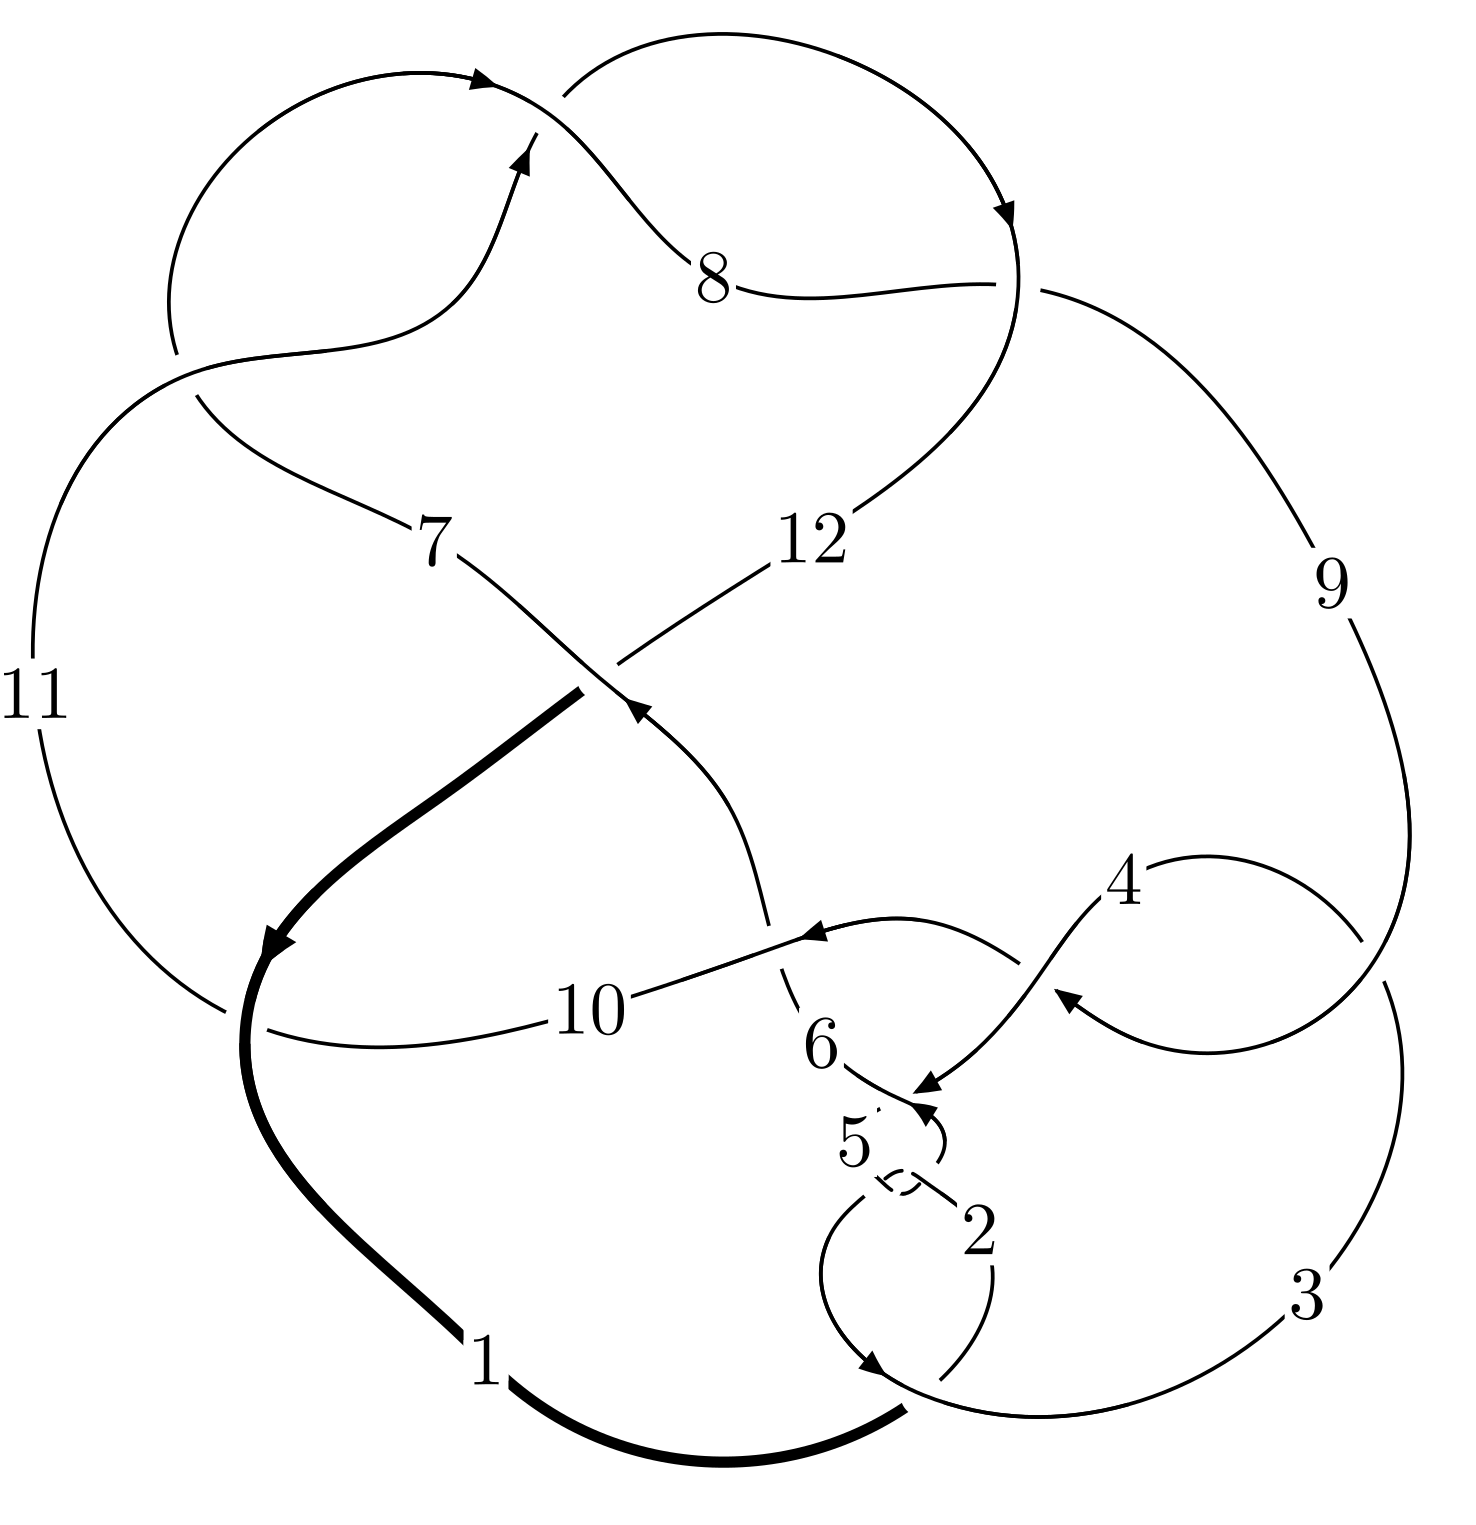
\includegraphics[width=112pt]{../../../GIT/diagram.site/Diagrams/png/974_12a_0173.png}\\
\ \ \ A knot diagram\footnotemark}&
\allowdisplaybreaks
\textbf{Linearized knot diagam} \\
\cline{2-2}
 &
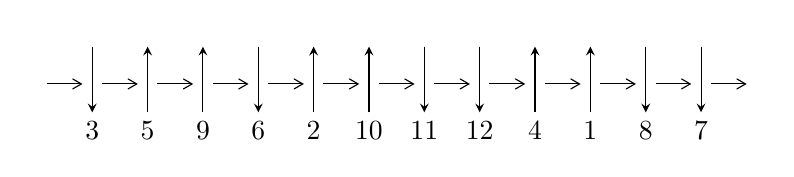
\begin{tikzpicture}[x=20pt, y=17pt]
	% nodes
	\node (C0) at (0, 0) {};
	\node (C1) at (1, 0) {};
	\node (C1U) at (1, +1) {};
	\node (C1D) at (1, -1) {3};

	\node (C2) at (2, 0) {};
	\node (C2U) at (2, +1) {};
	\node (C2D) at (2, -1) {5};

	\node (C3) at (3, 0) {};
	\node (C3U) at (3, +1) {};
	\node (C3D) at (3, -1) {9};

	\node (C4) at (4, 0) {};
	\node (C4U) at (4, +1) {};
	\node (C4D) at (4, -1) {6};

	\node (C5) at (5, 0) {};
	\node (C5U) at (5, +1) {};
	\node (C5D) at (5, -1) {2};

	\node (C6) at (6, 0) {};
	\node (C6U) at (6, +1) {};
	\node (C6D) at (6, -1) {10};

	\node (C7) at (7, 0) {};
	\node (C7U) at (7, +1) {};
	\node (C7D) at (7, -1) {11};

	\node (C8) at (8, 0) {};
	\node (C8U) at (8, +1) {};
	\node (C8D) at (8, -1) {12};

	\node (C9) at (9, 0) {};
	\node (C9U) at (9, +1) {};
	\node (C9D) at (9, -1) {4};

	\node (C10) at (10, 0) {};
	\node (C10U) at (10, +1) {};
	\node (C10D) at (10, -1) {1};

	\node (C11) at (11, 0) {};
	\node (C11U) at (11, +1) {};
	\node (C11D) at (11, -1) {8};

	\node (C12) at (12, 0) {};
	\node (C12U) at (12, +1) {};
	\node (C12D) at (12, -1) {7};
	\node (C13) at (13, 0) {};

	% arrows
	\draw[->,>={angle 60}]
	(C0) edge (C1) (C1) edge (C2) (C2) edge (C3) (C3) edge (C4) (C4) edge (C5) (C5) edge (C6) (C6) edge (C7) (C7) edge (C8) (C8) edge (C9) (C9) edge (C10) (C10) edge (C11) (C11) edge (C12) (C12) edge (C13) ;	\draw[->,>=stealth]
	(C1U) edge (C1D) (C2D) edge (C2U) (C3D) edge (C3U) (C4U) edge (C4D) (C5D) edge (C5U) (C6D) edge (C6U) (C7U) edge (C7D) (C8U) edge (C8D) (C9D) edge (C9U) (C10D) edge (C10U) (C11U) edge (C11D) (C12U) edge (C12D) ;
	\end{tikzpicture} \\
\hhline{~~} \\& 
\textbf{Solving Sequence} \\ \cline{2-2} 
 &
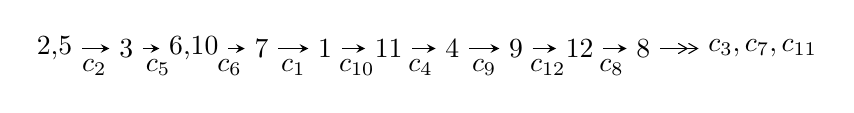
\begin{tikzpicture}[x=23pt, y=7pt]
	% node
	\node (A0) at (-1/8, 0) {2,5};
	\node (A1) at (1, 0) {3};
	\node (A2) at (33/16, 0) {6,10};
	\node (A3) at (25/8, 0) {7};
	\node (A4) at (33/8, 0) {1};
	\node (A5) at (41/8, 0) {11};
	\node (A6) at (49/8, 0) {4};
	\node (A7) at (57/8, 0) {9};
	\node (A8) at (65/8, 0) {12};
	\node (A9) at (73/8, 0) {8};
	\node (C1) at (1/2, -1) {$c_{2}$};
	\node (C2) at (3/2, -1) {$c_{5}$};
	\node (C3) at (21/8, -1) {$c_{6}$};
	\node (C4) at (29/8, -1) {$c_{1}$};
	\node (C5) at (37/8, -1) {$c_{10}$};
	\node (C6) at (45/8, -1) {$c_{4}$};
	\node (C7) at (53/8, -1) {$c_{9}$};
	\node (C8) at (61/8, -1) {$c_{12}$};
	\node (C9) at (69/8, -1) {$c_{8}$};
	\node (A10) at (11, 0) {$c_{3},c_{7},c_{11}$};

	% edge
	\draw[->,>=stealth]	
	(A0) edge (A1) (A1) edge (A2) (A2) edge (A3) (A3) edge (A4) (A4) edge (A5) (A5) edge (A6) (A6) edge (A7) (A7) edge (A8) (A8) edge (A9) ;
	\draw[->>,>={angle 60}]	
	(A9) edge (A10);
\end{tikzpicture} \\ 

\end{tabular} \\

\footnotetext{
The image of knot diagram is generated by the software ``\textbf{Draw programme}" developed by Andrew Bartholomew(\url{http://www.layer8.co.uk/maths/draw/index.htm\#Running-draw}), where we modified some parts for our purpose(\url{https://github.com/CATsTAILs/LinksPainter}).
}\phantom \\ \newline 
\centering \textbf{Ideals for irreducible components\footnotemark of $X_{\text{par}}$} 
 
\begin{align*}
I^u_{1}&=\langle 
222 u^{93}-751 u^{92}+\cdots+16 b+223,\;333 u^{93}-1867 u^{92}+\cdots+16 a-288,\;u^{94}-6 u^{93}+\cdots-7 u+1\rangle \\
I^u_{2}&=\langle 
- a u+b- a,\;a^5- a^4 u-2 a^3 u-2 a^3- a^2+a u+u+1,\;u^2+u+1\rangle \\
\\
\end{align*}
\raggedright * 2 irreducible components of $\dim_{\mathbb{C}}=0$, with total 104 representations.\\
\footnotetext{All coefficients of polynomials are rational numbers. But the coefficients are sometimes approximated in decimal forms when there is not enough margin.}
\newpage
\renewcommand{\arraystretch}{1}
\centering \section*{I. $I^u_{1}= \langle 222 u^{93}-751 u^{92}+\cdots+16 b+223,\;333 u^{93}-1867 u^{92}+\cdots+16 a-288,\;u^{94}-6 u^{93}+\cdots-7 u+1 \rangle$}
\flushleft \textbf{(i) Arc colorings}\\
\begin{tabular}{m{7pt} m{180pt} m{7pt} m{180pt} }
\flushright $a_{2}=$&$\begin{pmatrix}1\\0\end{pmatrix}$ \\
\flushright $a_{5}=$&$\begin{pmatrix}0\\u\end{pmatrix}$ \\
\flushright $a_{3}=$&$\begin{pmatrix}1\\- u^2\end{pmatrix}$ \\
\flushright $a_{6}=$&$\begin{pmatrix}u\\u\end{pmatrix}$ \\
\flushright $a_{10}=$&$\begin{pmatrix}-20.8125 u^{93}+116.688 u^{92}+\cdots-123.813 u+18\\-13.8750 u^{93}+46.9375 u^{92}+\cdots+67.8750 u-13.9375\end{pmatrix}$ \\
\flushright $a_{7}=$&$\begin{pmatrix}\frac{1}{16} u^{93}-\frac{3}{8} u^{92}+\cdots+\frac{7}{16} u-\frac{17}{16}\\0.0625000 u^{93}-0.312500 u^{92}+\cdots+2.62500 u^{2}+2.06250 u\end{pmatrix}$ \\
\flushright $a_{1}=$&$\begin{pmatrix}u^2+1\\- u^4\end{pmatrix}$ \\
\flushright $a_{11}=$&$\begin{pmatrix}-\frac{655}{8} u^{93}+450 u^{92}+\cdots-\frac{3365}{8} u+\frac{481}{8}\\-79.1875 u^{93}+363.500 u^{92}+\cdots-71.1875 u+1.18750\end{pmatrix}$ \\
\flushright $a_{4}=$&$\begin{pmatrix}u^3\\u^3+u\end{pmatrix}$ \\
\flushright $a_{9}=$&$\begin{pmatrix}-65.9375 u^{93}+362.563 u^{92}+\cdots-346.688 u+50\\-60.1250 u^{93}+267.563 u^{92}+\cdots-15.1250 u-5.81250\end{pmatrix}$ \\
\flushright $a_{12}=$&$\begin{pmatrix}\frac{3}{8} u^{93}-\frac{9}{16} u^{92}+\cdots-\frac{43}{8} u+\frac{37}{16}\\-1.43750 u^{93}+8.93750 u^{92}+\cdots-12.5625 u+1.87500\end{pmatrix}$ \\
\flushright $a_{8}=$&$\begin{pmatrix}-0.812500 u^{93}+1.75000 u^{92}+\cdots+10.8125 u-2.31250\\\frac{9}{8} u^{93}-\frac{67}{8} u^{92}+\cdots+\frac{153}{8} u-\frac{23}{8}\end{pmatrix}$\\&\end{tabular}
\flushleft \textbf{(ii) Obstruction class $= -1$}\\~\\
\flushleft \textbf{(iii) Cusp Shapes $= -\frac{629}{16} u^{93}+\frac{2099}{16} u^{92}+\cdots+\frac{3621}{16} u-\frac{87}{2}$}\\~\\
\newpage\renewcommand{\arraystretch}{1}
\flushleft \textbf{(iv) u-Polynomials at the component}\newline \\
\begin{tabular}{m{50pt}|m{274pt}}
Crossings & \hspace{64pt}u-Polynomials at each crossing \\
\hline $$\begin{aligned}c_{1},c_{4}\end{aligned}$$&$\begin{aligned}
&u^{94}+30 u^{93}+\cdots- u+1
\end{aligned}$\\
\hline $$\begin{aligned}c_{2},c_{5}\end{aligned}$$&$\begin{aligned}
&u^{94}+6 u^{93}+\cdots+7 u+1
\end{aligned}$\\
\hline $$\begin{aligned}c_{3},c_{9}\end{aligned}$$&$\begin{aligned}
&u^{94}+u^{93}+\cdots+3072 u+1024
\end{aligned}$\\
\hline $$\begin{aligned}c_{6}\end{aligned}$$&$\begin{aligned}
&u^{94}-3 u^{93}+\cdots-87286 u+32129
\end{aligned}$\\
\hline $$\begin{aligned}c_{7},c_{8},c_{11}\end{aligned}$$&$\begin{aligned}
&u^{94}+3 u^{93}+\cdots-2 u+1
\end{aligned}$\\
\hline $$\begin{aligned}c_{10}\end{aligned}$$&$\begin{aligned}
&u^{94}+21 u^{93}+\cdots+36030 u+2513
\end{aligned}$\\
\hline $$\begin{aligned}c_{12}\end{aligned}$$&$\begin{aligned}
&u^{94}-9 u^{93}+\cdots-6 u+1
\end{aligned}$\\
\hline
\end{tabular}\\~\\
\newpage\renewcommand{\arraystretch}{1}
\flushleft \textbf{(v) Riley Polynomials at the component}\newline \\
\begin{tabular}{m{50pt}|m{274pt}}
Crossings & \hspace{64pt}Riley Polynomials at each crossing \\
\hline $$\begin{aligned}c_{1},c_{4}\end{aligned}$$&$\begin{aligned}
&y^{94}+74 y^{93}+\cdots+351 y+1
\end{aligned}$\\
\hline $$\begin{aligned}c_{2},c_{5}\end{aligned}$$&$\begin{aligned}
&y^{94}+30 y^{93}+\cdots- y+1
\end{aligned}$\\
\hline $$\begin{aligned}c_{3},c_{9}\end{aligned}$$&$\begin{aligned}
&y^{94}-55 y^{93}+\cdots-14680064 y+1048576
\end{aligned}$\\
\hline $$\begin{aligned}c_{6}\end{aligned}$$&$\begin{aligned}
&y^{94}-37 y^{93}+\cdots+47515546332 y+1032272641
\end{aligned}$\\
\hline $$\begin{aligned}c_{7},c_{8},c_{11}\end{aligned}$$&$\begin{aligned}
&y^{94}-85 y^{93}+\cdots+8 y+1
\end{aligned}$\\
\hline $$\begin{aligned}c_{10}\end{aligned}$$&$\begin{aligned}
&y^{94}+23 y^{93}+\cdots+134228996 y+6315169
\end{aligned}$\\
\hline $$\begin{aligned}c_{12}\end{aligned}$$&$\begin{aligned}
&y^{94}- y^{93}+\cdots-4 y+1
\end{aligned}$\\
\hline
\end{tabular}\\~\\
\newpage\flushleft \textbf{(vi) Complex Volumes and Cusp Shapes}
$$\begin{array}{c|c|c}  
\text{Solutions to }I^u_{1}& \I (\text{vol} + \sqrt{-1}CS) & \text{Cusp shape}\\
 \hline 
\begin{aligned}
u &= -0.670150 + 0.687540 I \\
a &= \phantom{-}1.51532 - 0.23955 I \\
b &= \phantom{-}1.43637 + 0.41065 I\end{aligned}
 & -3.59197 - 3.38028 I & \phantom{-0.000000 } 0 \\ \hline\begin{aligned}
u &= -0.670150 - 0.687540 I \\
a &= \phantom{-}1.51532 + 0.23955 I \\
b &= \phantom{-}1.43637 - 0.41065 I\end{aligned}
 & -3.59197 + 3.38028 I & \phantom{-0.000000 } 0 \\ \hline\begin{aligned}
u &= \phantom{-}0.028187 + 0.943205 I \\
a &= \phantom{-}0.485350 - 1.000310 I \\
b &= -0.859995 - 0.725734 I\end{aligned}
 & -8.40957 - 3.13792 I & \phantom{-0.000000 } 0 \\ \hline\begin{aligned}
u &= \phantom{-}0.028187 - 0.943205 I \\
a &= \phantom{-}0.485350 + 1.000310 I \\
b &= -0.859995 + 0.725734 I\end{aligned}
 & -8.40957 + 3.13792 I & \phantom{-0.000000 } 0 \\ \hline\begin{aligned}
u &= -0.148866 + 1.063320 I \\
a &= \phantom{-}0.294932 + 0.195503 I \\
b &= -0.709994 - 0.403961 I\end{aligned}
 & -7.43720 - 1.60373 I & \phantom{-0.000000 } 0 \\ \hline\begin{aligned}
u &= -0.148866 - 1.063320 I \\
a &= \phantom{-}0.294932 - 0.195503 I \\
b &= -0.709994 + 0.403961 I\end{aligned}
 & -7.43720 + 1.60373 I & \phantom{-0.000000 } 0 \\ \hline\begin{aligned}
u &= -0.227030 + 1.053750 I \\
a &= \phantom{-}0.164857 - 0.261042 I \\
b &= \phantom{-}0.835518 + 0.426311 I\end{aligned}
 & -1.39198 - 3.10591 I & \phantom{-0.000000 } 0 \\ \hline\begin{aligned}
u &= -0.227030 - 1.053750 I \\
a &= \phantom{-}0.164857 + 0.261042 I \\
b &= \phantom{-}0.835518 - 0.426311 I\end{aligned}
 & -1.39198 + 3.10591 I & \phantom{-0.000000 } 0 \\ \hline\begin{aligned}
u &= -0.516749 + 0.947808 I \\
a &= \phantom{-}0.371632 + 0.718636 I \\
b &= \phantom{-}0.054881 + 0.933589 I\end{aligned}
 & -0.12135 - 2.69520 I & \phantom{-0.000000 } 0 \\ \hline\begin{aligned}
u &= -0.516749 - 0.947808 I \\
a &= \phantom{-}0.371632 - 0.718636 I \\
b &= \phantom{-}0.054881 - 0.933589 I\end{aligned}
 & -0.12135 + 2.69520 I & \phantom{-0.000000 } 0\\
 \hline 
 \end{array}$$\newpage$$\begin{array}{c|c|c}  
\text{Solutions to }I^u_{1}& \I (\text{vol} + \sqrt{-1}CS) & \text{Cusp shape}\\
 \hline 
\begin{aligned}
u &= \phantom{-}0.681660 + 0.840872 I \\
a &= \phantom{-}1.284810 - 0.135715 I \\
b &= \phantom{-}0.30599 - 1.51899 I\end{aligned}
 & -4.62497 - 2.25618 I & \phantom{-0.000000 } 0 \\ \hline\begin{aligned}
u &= \phantom{-}0.681660 - 0.840872 I \\
a &= \phantom{-}1.284810 + 0.135715 I \\
b &= \phantom{-}0.30599 + 1.51899 I\end{aligned}
 & -4.62497 + 2.25618 I & \phantom{-0.000000 } 0 \\ \hline\begin{aligned}
u &= \phantom{-}0.820354 + 0.710067 I \\
a &= \phantom{-}1.19044 + 1.34503 I \\
b &= \phantom{-}1.63767 - 0.08811 I\end{aligned}
 & -0.86724 - 1.44181 I & \phantom{-0.000000 } 0 \\ \hline\begin{aligned}
u &= \phantom{-}0.820354 - 0.710067 I \\
a &= \phantom{-}1.19044 - 1.34503 I \\
b &= \phantom{-}1.63767 + 0.08811 I\end{aligned}
 & -0.86724 + 1.44181 I & \phantom{-0.000000 } 0 \\ \hline\begin{aligned}
u &= -0.301226 + 1.064560 I \\
a &= \phantom{-}0.572796 - 0.267999 I \\
b &= \phantom{-}0.945557 + 0.533013 I\end{aligned}
 & -1.28046 - 3.45860 I & \phantom{-0.000000 } 0 \\ \hline\begin{aligned}
u &= -0.301226 - 1.064560 I \\
a &= \phantom{-}0.572796 + 0.267999 I \\
b &= \phantom{-}0.945557 - 0.533013 I\end{aligned}
 & -1.28046 + 3.45860 I & \phantom{-0.000000 } 0 \\ \hline\begin{aligned}
u &= -0.773091 + 0.795511 I \\
a &= -2.04021 + 1.13036 I \\
b &= -2.43499 + 0.17340 I\end{aligned}
 & -1.66418 + 4.07578 I & \phantom{-0.000000 } 0 \\ \hline\begin{aligned}
u &= -0.773091 - 0.795511 I \\
a &= -2.04021 - 1.13036 I \\
b &= -2.43499 - 0.17340 I\end{aligned}
 & -1.66418 - 4.07578 I & \phantom{-0.000000 } 0 \\ \hline\begin{aligned}
u &= \phantom{-}0.707009 + 0.855951 I \\
a &= -0.916465 + 0.148403 I \\
b &= -0.029416 + 1.238170 I\end{aligned}
 & \phantom{-}1.39464 + 0.74314 I & \phantom{-0.000000 } 0 \\ \hline\begin{aligned}
u &= \phantom{-}0.707009 - 0.855951 I \\
a &= -0.916465 - 0.148403 I \\
b &= -0.029416 - 1.238170 I\end{aligned}
 & \phantom{-}1.39464 - 0.74314 I & \phantom{-0.000000 } 0\\
 \hline 
 \end{array}$$\newpage$$\begin{array}{c|c|c}  
\text{Solutions to }I^u_{1}& \I (\text{vol} + \sqrt{-1}CS) & \text{Cusp shape}\\
 \hline 
\begin{aligned}
u &= -0.758040 + 0.817422 I \\
a &= \phantom{-}1.84855 - 1.28828 I \\
b &= \phantom{-}2.31971 - 0.42290 I\end{aligned}
 & \phantom{-}3.44140 + 0.58481 I & \phantom{-0.000000 } 0 \\ \hline\begin{aligned}
u &= -0.758040 - 0.817422 I \\
a &= \phantom{-}1.84855 + 1.28828 I \\
b &= \phantom{-}2.31971 + 0.42290 I\end{aligned}
 & \phantom{-}3.44140 - 0.58481 I & \phantom{-0.000000 } 0 \\ \hline\begin{aligned}
u &= \phantom{-}0.129795 + 0.870515 I \\
a &= -0.20956 + 1.60326 I \\
b &= \phantom{-}1.21590 + 0.76608 I\end{aligned}
 & -7.30094 + 5.76750 I & \phantom{-0.000000 } 0 \\ \hline\begin{aligned}
u &= \phantom{-}0.129795 - 0.870515 I \\
a &= -0.20956 - 1.60326 I \\
b &= \phantom{-}1.21590 - 0.76608 I\end{aligned}
 & -7.30094 - 5.76750 I & \phantom{-0.000000 } 0 \\ \hline\begin{aligned}
u &= -0.390296 + 1.052370 I \\
a &= -0.917390 - 0.070137 I \\
b &= -0.916064 - 0.825313 I\end{aligned}
 & \phantom{-}1.057540 - 0.415655 I & \phantom{-0.000000 } 0 \\ \hline\begin{aligned}
u &= -0.390296 - 1.052370 I \\
a &= -0.917390 + 0.070137 I \\
b &= -0.916064 + 0.825313 I\end{aligned}
 & \phantom{-}1.057540 + 0.415655 I & \phantom{-0.000000 } 0 \\ \hline\begin{aligned}
u &= \phantom{-}0.881750 + 0.696556 I \\
a &= -1.30206 - 1.74356 I \\
b &= -2.09845 - 0.37324 I\end{aligned}
 & \phantom{-}2.09884 - 10.39320 I & \phantom{-0.000000 } 0 \\ \hline\begin{aligned}
u &= \phantom{-}0.881750 - 0.696556 I \\
a &= -1.30206 + 1.74356 I \\
b &= -2.09845 + 0.37324 I\end{aligned}
 & \phantom{-}2.09884 + 10.39320 I & \phantom{-0.000000 } 0 \\ \hline\begin{aligned}
u &= \phantom{-}0.861955 + 0.728574 I \\
a &= -1.04499 - 1.61989 I \\
b &= -1.66754 - 0.38829 I\end{aligned}
 & \phantom{-}5.87498 - 2.63356 I & \phantom{-0.000000 } 0 \\ \hline\begin{aligned}
u &= \phantom{-}0.861955 - 0.728574 I \\
a &= -1.04499 + 1.61989 I \\
b &= -1.66754 + 0.38829 I\end{aligned}
 & \phantom{-}5.87498 + 2.63356 I & \phantom{-0.000000 } 0\\
 \hline 
 \end{array}$$\newpage$$\begin{array}{c|c|c}  
\text{Solutions to }I^u_{1}& \I (\text{vol} + \sqrt{-1}CS) & \text{Cusp shape}\\
 \hline 
\begin{aligned}
u &= \phantom{-}0.877643 + 0.710110 I \\
a &= \phantom{-}1.19562 + 1.73143 I \\
b &= \phantom{-}1.94503 + 0.42864 I\end{aligned}
 & \phantom{-}7.48515 - 6.65000 I & \phantom{-0.000000 } 0 \\ \hline\begin{aligned}
u &= \phantom{-}0.877643 - 0.710110 I \\
a &= \phantom{-}1.19562 - 1.73143 I \\
b &= \phantom{-}1.94503 - 0.42864 I\end{aligned}
 & \phantom{-}7.48515 + 6.65000 I & \phantom{-0.000000 } 0 \\ \hline\begin{aligned}
u &= -0.222597 + 1.109100 I \\
a &= -0.114066 + 0.610663 I \\
b &= -0.877550 - 0.310159 I\end{aligned}
 & \phantom{-}0.03457 - 6.69622 I & \phantom{-0.000000 } 0 \\ \hline\begin{aligned}
u &= -0.222597 - 1.109100 I \\
a &= -0.114066 - 0.610663 I \\
b &= -0.877550 + 0.310159 I\end{aligned}
 & \phantom{-}0.03457 + 6.69622 I & \phantom{-0.000000 } 0 \\ \hline\begin{aligned}
u &= \phantom{-}0.682317 + 0.903998 I \\
a &= -0.830811 + 0.899927 I \\
b &= \phantom{-}0.57217 + 1.71044 I\end{aligned}
 & -4.82787 + 7.52028 I & \phantom{-0.000000 } 0 \\ \hline\begin{aligned}
u &= \phantom{-}0.682317 - 0.903998 I \\
a &= -0.830811 - 0.899927 I \\
b &= \phantom{-}0.57217 - 1.71044 I\end{aligned}
 & -4.82787 - 7.52028 I & \phantom{-0.000000 } 0 \\ \hline\begin{aligned}
u &= \phantom{-}0.005767 + 0.865357 I \\
a &= -0.095106 + 1.029290 I \\
b &= \phantom{-}0.952216 + 0.583554 I\end{aligned}
 & -2.52879 - 0.93392 I & \phantom{-0.000000 } 0 \\ \hline\begin{aligned}
u &= \phantom{-}0.005767 - 0.865357 I \\
a &= -0.095106 - 1.029290 I \\
b &= \phantom{-}0.952216 - 0.583554 I\end{aligned}
 & -2.52879 + 0.93392 I & \phantom{-0.000000 } 0 \\ \hline\begin{aligned}
u &= \phantom{-}0.706391 + 0.890180 I \\
a &= \phantom{-}0.661512 - 0.528645 I \\
b &= -0.436068 - 1.333350 I\end{aligned}
 & \phantom{-}1.28701 + 4.67596 I & \phantom{-0.000000 } 0 \\ \hline\begin{aligned}
u &= \phantom{-}0.706391 - 0.890180 I \\
a &= \phantom{-}0.661512 + 0.528645 I \\
b &= -0.436068 + 1.333350 I\end{aligned}
 & \phantom{-}1.28701 - 4.67596 I & \phantom{-0.000000 } 0\\
 \hline 
 \end{array}$$\newpage$$\begin{array}{c|c|c}  
\text{Solutions to }I^u_{1}& \I (\text{vol} + \sqrt{-1}CS) & \text{Cusp shape}\\
 \hline 
\begin{aligned}
u &= -0.717761 + 0.883186 I \\
a &= -1.20707 + 1.68520 I \\
b &= -1.88096 + 1.10363 I\end{aligned}
 & \phantom{-}1.33806 - 2.75239 I & \phantom{-0.000000 } 0 \\ \hline\begin{aligned}
u &= -0.717761 - 0.883186 I \\
a &= -1.20707 - 1.68520 I \\
b &= -1.88096 - 1.10363 I\end{aligned}
 & \phantom{-}1.33806 + 2.75239 I & \phantom{-0.000000 } 0 \\ \hline\begin{aligned}
u &= -0.737938 + 0.867429 I \\
a &= -1.46729 + 1.65641 I \\
b &= -2.11782 + 0.95891 I\end{aligned}
 & \phantom{-}1.36896 - 2.79585 I & \phantom{-0.000000 } 0 \\ \hline\begin{aligned}
u &= -0.737938 - 0.867429 I \\
a &= -1.46729 - 1.65641 I \\
b &= -2.11782 - 0.95891 I\end{aligned}
 & \phantom{-}1.36896 + 2.79585 I & \phantom{-0.000000 } 0 \\ \hline\begin{aligned}
u &= -0.208400 + 1.126740 I \\
a &= -0.004628 - 0.735193 I \\
b &= \phantom{-}0.850790 + 0.246650 I\end{aligned}
 & -5.32826 - 10.21790 I & \phantom{-0.000000 } 0 \\ \hline\begin{aligned}
u &= -0.208400 - 1.126740 I \\
a &= -0.004628 + 0.735193 I \\
b &= \phantom{-}0.850790 - 0.246650 I\end{aligned}
 & -5.32826 + 10.21790 I & \phantom{-0.000000 } 0 \\ \hline\begin{aligned}
u &= -0.524352 + 1.021570 I \\
a &= -0.860237 - 0.944500 I \\
b &= -0.35864 - 1.40193 I\end{aligned}
 & -5.23793 - 4.84037 I & \phantom{-0.000000 } 0 \\ \hline\begin{aligned}
u &= -0.524352 - 1.021570 I \\
a &= -0.860237 + 0.944500 I \\
b &= -0.35864 + 1.40193 I\end{aligned}
 & -5.23793 + 4.84037 I & \phantom{-0.000000 } 0 \\ \hline\begin{aligned}
u &= \phantom{-}0.866098 + 0.763349 I \\
a &= -0.74715 - 1.63566 I \\
b &= -1.30988 - 0.62048 I\end{aligned}
 & \phantom{-}6.43442 - 2.50562 I & \phantom{-0.000000 } 0 \\ \hline\begin{aligned}
u &= \phantom{-}0.866098 - 0.763349 I \\
a &= -0.74715 + 1.63566 I \\
b &= -1.30988 + 0.62048 I\end{aligned}
 & \phantom{-}6.43442 + 2.50562 I & \phantom{-0.000000 } 0\\
 \hline 
 \end{array}$$\newpage$$\begin{array}{c|c|c}  
\text{Solutions to }I^u_{1}& \I (\text{vol} + \sqrt{-1}CS) & \text{Cusp shape}\\
 \hline 
\begin{aligned}
u &= \phantom{-}0.095033 + 0.837949 I \\
a &= \phantom{-}0.04708 - 1.43600 I \\
b &= -1.161730 - 0.628848 I\end{aligned}
 & -1.75593 + 2.53049 I & \phantom{-0.000000 } 0 \\ \hline\begin{aligned}
u &= \phantom{-}0.095033 - 0.837949 I \\
a &= \phantom{-}0.04708 + 1.43600 I \\
b &= -1.161730 + 0.628848 I\end{aligned}
 & -1.75593 - 2.53049 I & \phantom{-0.000000 } 0 \\ \hline\begin{aligned}
u &= -0.424352 + 1.076360 I \\
a &= \phantom{-}1.157350 + 0.174838 I \\
b &= \phantom{-}0.99354 + 1.01112 I\end{aligned}
 & -4.02052 + 2.87938 I & \phantom{-0.000000 } 0 \\ \hline\begin{aligned}
u &= -0.424352 - 1.076360 I \\
a &= \phantom{-}1.157350 - 0.174838 I \\
b &= \phantom{-}0.99354 - 1.01112 I\end{aligned}
 & -4.02052 - 2.87938 I & \phantom{-0.000000 } 0 \\ \hline\begin{aligned}
u &= -0.658896 + 0.954952 I \\
a &= \phantom{-}0.25075 - 1.81159 I \\
b &= \phantom{-}1.04116 - 1.64540 I\end{aligned}
 & -4.36826 - 1.76808 I & \phantom{-0.000000 } 0 \\ \hline\begin{aligned}
u &= -0.658896 - 0.954952 I \\
a &= \phantom{-}0.25075 + 1.81159 I \\
b &= \phantom{-}1.04116 + 1.64540 I\end{aligned}
 & -4.36826 + 1.76808 I & \phantom{-0.000000 } 0 \\ \hline\begin{aligned}
u &= \phantom{-}0.860409 + 0.792585 I \\
a &= \phantom{-}0.47498 + 1.53086 I \\
b &= \phantom{-}0.921903 + 0.686814 I\end{aligned}
 & \phantom{-}9.09436 + 1.27268 I & \phantom{-0.000000 } 0 \\ \hline\begin{aligned}
u &= \phantom{-}0.860409 - 0.792585 I \\
a &= \phantom{-}0.47498 - 1.53086 I \\
b &= \phantom{-}0.921903 - 0.686814 I\end{aligned}
 & \phantom{-}9.09436 - 1.27268 I & \phantom{-0.000000 } 0 \\ \hline\begin{aligned}
u &= \phantom{-}0.856194 + 0.815572 I \\
a &= -0.24752 - 1.42122 I \\
b &= -0.597569 - 0.719094 I\end{aligned}
 & \phantom{-}4.41649 + 4.98775 I & \phantom{-0.000000 } 0 \\ \hline\begin{aligned}
u &= \phantom{-}0.856194 - 0.815572 I \\
a &= -0.24752 + 1.42122 I \\
b &= -0.597569 + 0.719094 I\end{aligned}
 & \phantom{-}4.41649 - 4.98775 I & \phantom{-0.000000 } 0\\
 \hline 
 \end{array}$$\newpage$$\begin{array}{c|c|c}  
\text{Solutions to }I^u_{1}& \I (\text{vol} + \sqrt{-1}CS) & \text{Cusp shape}\\
 \hline 
\begin{aligned}
u &= -0.737336 + 0.926535 I \\
a &= \phantom{-}1.10299 - 2.19955 I \\
b &= \phantom{-}2.00654 - 1.63952 I\end{aligned}
 & \phantom{-}3.10639 - 6.25660 I & \phantom{-0.000000 } 0 \\ \hline\begin{aligned}
u &= -0.737336 - 0.926535 I \\
a &= \phantom{-}1.10299 + 2.19955 I \\
b &= \phantom{-}2.00654 + 1.63952 I\end{aligned}
 & \phantom{-}3.10639 + 6.25660 I & \phantom{-0.000000 } 0 \\ \hline\begin{aligned}
u &= -0.739971 + 0.944705 I \\
a &= -0.99082 + 2.39371 I \\
b &= -1.98203 + 1.87142 I\end{aligned}
 & -2.12113 - 9.79929 I & \phantom{-0.000000 } 0 \\ \hline\begin{aligned}
u &= -0.739971 - 0.944705 I \\
a &= -0.99082 - 2.39371 I \\
b &= -1.98203 - 1.87142 I\end{aligned}
 & -2.12113 + 9.79929 I & \phantom{-0.000000 } 0 \\ \hline\begin{aligned}
u &= -0.460070 + 0.644601 I \\
a &= -0.981985 - 0.230514 I \\
b &= -0.782718 - 0.369925 I\end{aligned}
 & \phantom{-}0.76337 - 1.37281 I & \phantom{-}5.90020 + 4.40804 I \\ \hline\begin{aligned}
u &= -0.460070 - 0.644601 I \\
a &= -0.981985 + 0.230514 I \\
b &= -0.782718 + 0.369925 I\end{aligned}
 & \phantom{-}0.76337 + 1.37281 I & \phantom{-}5.90020 - 4.40804 I \\ \hline\begin{aligned}
u &= -0.778683 + 0.137337 I \\
a &= -0.712517 - 0.452447 I \\
b &= \phantom{-}0.847873 - 0.744073 I\end{aligned}
 & -1.07737 - 7.05448 I & \phantom{-}2.24170 + 5.60574 I \\ \hline\begin{aligned}
u &= -0.778683 - 0.137337 I \\
a &= -0.712517 + 0.452447 I \\
b &= \phantom{-}0.847873 + 0.744073 I\end{aligned}
 & -1.07737 + 7.05448 I & \phantom{-}2.24170 - 5.60574 I \\ \hline\begin{aligned}
u &= -0.760762 + 0.101349 I \\
a &= \phantom{-}0.717928 + 0.321797 I \\
b &= -0.838743 + 0.523922 I\end{aligned}
 & \phantom{-}4.07426 - 3.50683 I & \phantom{-}7.35202 + 4.80092 I \\ \hline\begin{aligned}
u &= -0.760762 - 0.101349 I \\
a &= \phantom{-}0.717928 - 0.321797 I \\
b &= -0.838743 - 0.523922 I\end{aligned}
 & \phantom{-}4.07426 + 3.50683 I & \phantom{-}7.35202 - 4.80092 I\\
 \hline 
 \end{array}$$\newpage$$\begin{array}{c|c|c}  
\text{Solutions to }I^u_{1}& \I (\text{vol} + \sqrt{-1}CS) & \text{Cusp shape}\\
 \hline 
\begin{aligned}
u &= \phantom{-}0.735624 + 1.009360 I \\
a &= \phantom{-}0.89651 + 1.66114 I \\
b &= \phantom{-}2.23298 + 1.26801 I\end{aligned}
 & -1.78001 + 7.28363 I & \phantom{-0.000000 } 0 \\ \hline\begin{aligned}
u &= \phantom{-}0.735624 - 1.009360 I \\
a &= \phantom{-}0.89651 - 1.66114 I \\
b &= \phantom{-}2.23298 - 1.26801 I\end{aligned}
 & -1.78001 - 7.28363 I & \phantom{-0.000000 } 0 \\ \hline\begin{aligned}
u &= \phantom{-}0.799634 + 0.960875 I \\
a &= -1.093490 - 0.304083 I \\
b &= -1.70422 - 0.08876 I\end{aligned}
 & \phantom{-}3.96230 + 1.16547 I & \phantom{-0.000000 } 0 \\ \hline\begin{aligned}
u &= \phantom{-}0.799634 - 0.960875 I \\
a &= -1.093490 + 0.304083 I \\
b &= -1.70422 + 0.08876 I\end{aligned}
 & \phantom{-}3.96230 - 1.16547 I & \phantom{-0.000000 } 0 \\ \hline\begin{aligned}
u &= \phantom{-}0.790634 + 0.978809 I \\
a &= \phantom{-}1.222190 + 0.622146 I \\
b &= \phantom{-}1.97666 + 0.28955 I\end{aligned}
 & \phantom{-}8.51444 + 4.86478 I & \phantom{-0.000000 } 0 \\ \hline\begin{aligned}
u &= \phantom{-}0.790634 - 0.978809 I \\
a &= \phantom{-}1.222190 - 0.622146 I \\
b &= \phantom{-}1.97666 - 0.28955 I\end{aligned}
 & \phantom{-}8.51444 - 4.86478 I & \phantom{-0.000000 } 0 \\ \hline\begin{aligned}
u &= \phantom{-}0.780705 + 0.998864 I \\
a &= -1.35648 - 0.99279 I \\
b &= -2.27006 - 0.52715 I\end{aligned}
 & \phantom{-}5.70442 + 8.62660 I & \phantom{-0.000000 } 0 \\ \hline\begin{aligned}
u &= \phantom{-}0.780705 - 0.998864 I \\
a &= -1.35648 + 0.99279 I \\
b &= -2.27006 + 0.52715 I\end{aligned}
 & \phantom{-}5.70442 - 8.62660 I & \phantom{-0.000000 } 0 \\ \hline\begin{aligned}
u &= \phantom{-}0.760688 + 1.015770 I \\
a &= -1.30322 - 1.45901 I \\
b &= -2.44837 - 0.92304 I\end{aligned}
 & \phantom{-}4.98657 + 8.67496 I & \phantom{-0.000000 } 0 \\ \hline\begin{aligned}
u &= \phantom{-}0.760688 - 1.015770 I \\
a &= -1.30322 + 1.45901 I \\
b &= -2.44837 + 0.92304 I\end{aligned}
 & \phantom{-}4.98657 - 8.67496 I & \phantom{-0.000000 } 0\\
 \hline 
 \end{array}$$\newpage$$\begin{array}{c|c|c}  
\text{Solutions to }I^u_{1}& \I (\text{vol} + \sqrt{-1}CS) & \text{Cusp shape}\\
 \hline 
\begin{aligned}
u &= -0.722300 + 0.014530 I \\
a &= -0.781532 - 0.041951 I \\
b &= \phantom{-}0.742160 - 0.066804 I\end{aligned}
 & \phantom{-}2.12360 - 0.00608 I & \phantom{-}4.54516 - 0.30055 I \\ \hline\begin{aligned}
u &= -0.722300 - 0.014530 I \\
a &= -0.781532 + 0.041951 I \\
b &= \phantom{-}0.742160 + 0.066804 I\end{aligned}
 & \phantom{-}2.12360 + 0.00608 I & \phantom{-}4.54516 + 0.30055 I \\ \hline\begin{aligned}
u &= \phantom{-}0.760541 + 1.030980 I \\
a &= \phantom{-}1.48255 + 1.66923 I \\
b &= \phantom{-}2.68333 + 1.00565 I\end{aligned}
 & \phantom{-}6.4926 + 12.7332 I & \phantom{-0.000000 } 0 \\ \hline\begin{aligned}
u &= \phantom{-}0.760541 - 1.030980 I \\
a &= \phantom{-}1.48255 - 1.66923 I \\
b &= \phantom{-}2.68333 - 1.00565 I\end{aligned}
 & \phantom{-}6.4926 - 12.7332 I & \phantom{-0.000000 } 0 \\ \hline\begin{aligned}
u &= \phantom{-}0.756313 + 1.038710 I \\
a &= -1.51396 - 1.82875 I \\
b &= -2.77753 - 1.11565 I\end{aligned}
 & \phantom{-}1.0412 + 16.4719 I & \phantom{-0.000000 } 0 \\ \hline\begin{aligned}
u &= \phantom{-}0.756313 - 1.038710 I \\
a &= -1.51396 + 1.82875 I \\
b &= -2.77753 + 1.11565 I\end{aligned}
 & \phantom{-}1.0412 - 16.4719 I & \phantom{-0.000000 } 0 \\ \hline\begin{aligned}
u &= -0.585200 + 0.297480 I \\
a &= \phantom{-}1.221580 + 0.461509 I \\
b &= \phantom{-}0.173343 + 0.683235 I\end{aligned}
 & -3.34282 + 0.54984 I & -0.040630 + 1.106990 I \\ \hline\begin{aligned}
u &= -0.585200 - 0.297480 I \\
a &= \phantom{-}1.221580 - 0.461509 I \\
b &= \phantom{-}0.173343 - 0.683235 I\end{aligned}
 & -3.34282 - 0.54984 I & -0.040630 - 1.106990 I \\ \hline\begin{aligned}
u &= \phantom{-}0.061423 + 0.558350 I \\
a &= \phantom{-}0.79099 + 1.29367 I \\
b &= \phantom{-}1.011230 + 0.039242 I\end{aligned}
 & -2.80374 + 0.56424 I & -2.87695 + 0.40186 I \\ \hline\begin{aligned}
u &= \phantom{-}0.061423 - 0.558350 I \\
a &= \phantom{-}0.79099 - 1.29367 I \\
b &= \phantom{-}1.011230 - 0.039242 I\end{aligned}
 & -2.80374 - 0.56424 I & -2.87695 - 0.40186 I\\
 \hline 
 \end{array}$$\newpage$$\begin{array}{c|c|c}  
\text{Solutions to }I^u_{1}& \I (\text{vol} + \sqrt{-1}CS) & \text{Cusp shape}\\
 \hline 
\begin{aligned}
u &= \phantom{-}0.350629 + 0.139994 I \\
a &= \phantom{-}0.47125 + 1.44033 I \\
b &= \phantom{-}0.429853 - 1.025940 I\end{aligned}
 & -5.26747 - 4.05421 I & -4.34818 + 4.22545 I \\ \hline\begin{aligned}
u &= \phantom{-}0.350629 - 0.139994 I \\
a &= \phantom{-}0.47125 - 1.44033 I \\
b &= \phantom{-}0.429853 + 1.025940 I\end{aligned}
 & -5.26747 + 4.05421 I & -4.34818 - 4.22545 I \\ \hline\begin{aligned}
u &= \phantom{-}0.207313 + 0.143702 I \\
a &= -0.68341 - 1.86348 I \\
b &= -0.371998 + 0.632450 I\end{aligned}
 & -0.010818 - 1.279380 I & \phantom{-}0.07288 + 5.41961 I \\ \hline\begin{aligned}
u &= \phantom{-}0.207313 - 0.143702 I \\
a &= -0.68341 + 1.86348 I \\
b &= -0.371998 - 0.632450 I\end{aligned}
 & -0.010818 + 1.279380 I & \phantom{-}0.07288 - 5.41961 I\\
 \hline 
 \end{array}$$\newpage\newpage\renewcommand{\arraystretch}{1}
\centering \section*{II. $I^u_{2}= \langle - a u+b- a,\;a^5- a^4 u-2 a^3 u-2 a^3- a^2+a u+u+1,\;u^2+u+1 \rangle$}
\flushleft \textbf{(i) Arc colorings}\\
\begin{tabular}{m{7pt} m{180pt} m{7pt} m{180pt} }
\flushright $a_{2}=$&$\begin{pmatrix}1\\0\end{pmatrix}$ \\
\flushright $a_{5}=$&$\begin{pmatrix}0\\u\end{pmatrix}$ \\
\flushright $a_{3}=$&$\begin{pmatrix}1\\u+1\end{pmatrix}$ \\
\flushright $a_{6}=$&$\begin{pmatrix}u\\u\end{pmatrix}$ \\
\flushright $a_{10}=$&$\begin{pmatrix}a\\a u+a\end{pmatrix}$ \\
\flushright $a_{7}=$&$\begin{pmatrix}a^2 u+a^2+u\\a^2 u+u\end{pmatrix}$ \\
\flushright $a_{1}=$&$\begin{pmatrix}- u\\- u\end{pmatrix}$ \\
\flushright $a_{11}=$&$\begin{pmatrix}2 a\\a u+2 a\end{pmatrix}$ \\
\flushright $a_{4}=$&$\begin{pmatrix}1\\u+1\end{pmatrix}$ \\
\flushright $a_{9}=$&$\begin{pmatrix}a\\a u+a\end{pmatrix}$ \\
\flushright $a_{12}=$&$\begin{pmatrix}a^4+a^2 u+a^2- u\\a^4 u+a^4+a^2 u+a^2- u\end{pmatrix}$ \\
\flushright $a_{8}=$&$\begin{pmatrix}2 a^4- a^2 u- a^2+u\\a^4 u+2 a^4- a^2 u- a^2+u\end{pmatrix}$\\&\end{tabular}
\flushleft \textbf{(ii) Obstruction class $= 1$}\\~\\
\flushleft \textbf{(iii) Cusp Shapes $= - a^4+4 a^3-3 a^2 u-4 a u-5 a+4 u-2$}\\~\\
\newpage\renewcommand{\arraystretch}{1}
\flushleft \textbf{(iv) u-Polynomials at the component}\newline \\
\begin{tabular}{m{50pt}|m{274pt}}
Crossings & \hspace{64pt}u-Polynomials at each crossing \\
\hline $$\begin{aligned}c_{1},c_{4},c_{5}\end{aligned}$$&$\begin{aligned}
&(u^2- u+1)^5
\end{aligned}$\\
\hline $$\begin{aligned}c_{2}\end{aligned}$$&$\begin{aligned}
&(u^2+u+1)^5
\end{aligned}$\\
\hline $$\begin{aligned}c_{3},c_{9}\end{aligned}$$&$\begin{aligned}
&u^{10}
\end{aligned}$\\
\hline $$\begin{aligned}c_{6},c_{10}\end{aligned}$$&$\begin{aligned}
&(u^5- u^4+2 u^3- u^2+u-1)^2
\end{aligned}$\\
\hline $$\begin{aligned}c_{7},c_{8}\end{aligned}$$&$\begin{aligned}
&(u^5+u^4-2 u^3- u^2+u-1)^2
\end{aligned}$\\
\hline $$\begin{aligned}c_{11}\end{aligned}$$&$\begin{aligned}
&(u^5- u^4-2 u^3+u^2+u+1)^2
\end{aligned}$\\
\hline $$\begin{aligned}c_{12}\end{aligned}$$&$\begin{aligned}
&(u^5+3 u^4+4 u^3+u^2- u-1)^2
\end{aligned}$\\
\hline
\end{tabular}\\~\\
\newpage\renewcommand{\arraystretch}{1}
\flushleft \textbf{(v) Riley Polynomials at the component}\newline \\
\begin{tabular}{m{50pt}|m{274pt}}
Crossings & \hspace{64pt}Riley Polynomials at each crossing \\
\hline $$\begin{aligned}c_{1},c_{2},c_{4}\\c_{5}\end{aligned}$$&$\begin{aligned}
&(y^2+y+1)^5
\end{aligned}$\\
\hline $$\begin{aligned}c_{3},c_{9}\end{aligned}$$&$\begin{aligned}
&y^{10}
\end{aligned}$\\
\hline $$\begin{aligned}c_{6},c_{10}\end{aligned}$$&$\begin{aligned}
&(y^5+3 y^4+4 y^3+y^2- y-1)^2
\end{aligned}$\\
\hline $$\begin{aligned}c_{7},c_{8},c_{11}\end{aligned}$$&$\begin{aligned}
&(y^5-5 y^4+8 y^3-3 y^2- y-1)^2
\end{aligned}$\\
\hline $$\begin{aligned}c_{12}\end{aligned}$$&$\begin{aligned}
&(y^5- y^4+8 y^3-3 y^2+3 y-1)^2
\end{aligned}$\\
\hline
\end{tabular}\\~\\
\newpage\flushleft \textbf{(vi) Complex Volumes and Cusp Shapes}
$$\begin{array}{c|c|c}  
\text{Solutions to }I^u_{2}& \I (\text{vol} + \sqrt{-1}CS) & \text{Cusp shape}\\
 \hline 
\begin{aligned}
u &= -0.500000 + 0.866025 I \\
a &= \phantom{-}0.881753 + 0.117510 I \\
b &= \phantom{-}0.339110 + 0.822375 I\end{aligned}
 & -0.32910 - 3.56046 I & \phantom{-}0.01046 + 8.35149 I \\ \hline\begin{aligned}
u &= -0.500000 + 0.866025 I \\
a &= -0.542643 - 0.704866 I \\
b &= \phantom{-}0.339110 - 0.822375 I\end{aligned}
 & -0.329100 - 0.499304 I & -2.49844 - 0.84282 I \\ \hline\begin{aligned}
u &= -0.500000 + 0.866025 I \\
a &= -0.383413 + 0.664091 I \\
b &= -0.766826\phantom{ +0.000000I}\end{aligned}
 & -2.40108 - 2.02988 I & -0.33682 + 2.50057 I \\ \hline\begin{aligned}
u &= -0.500000 + 0.866025 I \\
a &= \phantom{-}0.811514 + 0.994721 I \\
b &= -0.455697 + 1.200150 I\end{aligned}
 & -5.87256 - 6.43072 I & -4.29156 + 5.94266 I \\ \hline\begin{aligned}
u &= -0.500000 + 0.866025 I \\
a &= -1.267210 - 0.205431 I \\
b &= -0.455697 - 1.200150 I\end{aligned}
 & -5.87256 + 2.37095 I & -6.88365 - 0.36343 I \\ \hline\begin{aligned}
u &= -0.500000 - 0.866025 I \\
a &= \phantom{-}0.881753 - 0.117510 I \\
b &= \phantom{-}0.339110 - 0.822375 I\end{aligned}
 & -0.32910 + 3.56046 I & \phantom{-}0.01046 - 8.35149 I \\ \hline\begin{aligned}
u &= -0.500000 - 0.866025 I \\
a &= -0.542643 + 0.704866 I \\
b &= \phantom{-}0.339110 + 0.822375 I\end{aligned}
 & -0.329100 + 0.499304 I & -2.49844 + 0.84282 I \\ \hline\begin{aligned}
u &= -0.500000 - 0.866025 I \\
a &= -0.383413 - 0.664091 I \\
b &= -0.766826\phantom{ +0.000000I}\end{aligned}
 & -2.40108 + 2.02988 I & -0.33682 - 2.50057 I \\ \hline\begin{aligned}
u &= -0.500000 - 0.866025 I \\
a &= \phantom{-}0.811514 - 0.994721 I \\
b &= -0.455697 - 1.200150 I\end{aligned}
 & -5.87256 + 6.43072 I & -4.29156 - 5.94266 I \\ \hline\begin{aligned}
u &= -0.500000 - 0.866025 I \\
a &= -1.267210 + 0.205431 I \\
b &= -0.455697 + 1.200150 I\end{aligned}
 & -5.87256 - 2.37095 I & -6.88365 + 0.36343 I\\
 \hline 
 \end{array}$$\newpage
\newpage\renewcommand{\arraystretch}{1}
\centering \section*{ III. u-Polynomials}
\begin{tabular}{m{50pt}|m{274pt}}
Crossings & \hspace{64pt}u-Polynomials at each crossing \\
\hline $$\begin{aligned}c_{1},c_{4}\end{aligned}$$&$\begin{aligned}
&((u^2- u+1)^5)(u^{94}+30 u^{93}+\cdots- u+1)
\end{aligned}$\\
\hline $$\begin{aligned}c_{2}\end{aligned}$$&$\begin{aligned}
&((u^2+u+1)^5)(u^{94}+6 u^{93}+\cdots+7 u+1)
\end{aligned}$\\
\hline $$\begin{aligned}c_{3},c_{9}\end{aligned}$$&$\begin{aligned}
&u^{10}(u^{94}+u^{93}+\cdots+3072 u+1024)
\end{aligned}$\\
\hline $$\begin{aligned}c_{5}\end{aligned}$$&$\begin{aligned}
&((u^2- u+1)^5)(u^{94}+6 u^{93}+\cdots+7 u+1)
\end{aligned}$\\
\hline $$\begin{aligned}c_{6}\end{aligned}$$&$\begin{aligned}
&((u^5- u^4+2 u^3- u^2+u-1)^2)(u^{94}-3 u^{93}+\cdots-87286 u+32129)
\end{aligned}$\\
\hline $$\begin{aligned}c_{7},c_{8}\end{aligned}$$&$\begin{aligned}
&((u^5+u^4-2 u^3- u^2+u-1)^2)(u^{94}+3 u^{93}+\cdots-2 u+1)
\end{aligned}$\\
\hline $$\begin{aligned}c_{10}\end{aligned}$$&$\begin{aligned}
&((u^5- u^4+2 u^3- u^2+u-1)^2)(u^{94}+21 u^{93}+\cdots+36030 u+2513)
\end{aligned}$\\
\hline $$\begin{aligned}c_{11}\end{aligned}$$&$\begin{aligned}
&((u^5- u^4-2 u^3+u^2+u+1)^2)(u^{94}+3 u^{93}+\cdots-2 u+1)
\end{aligned}$\\
\hline $$\begin{aligned}c_{12}\end{aligned}$$&$\begin{aligned}
&((u^5+3 u^4+4 u^3+u^2- u-1)^2)(u^{94}-9 u^{93}+\cdots-6 u+1)
\end{aligned}$\\
\hline
\end{tabular}\newpage\renewcommand{\arraystretch}{1}
\centering \section*{ IV. Riley Polynomials}
\begin{tabular}{m{50pt}|m{274pt}}
Crossings & \hspace{64pt}Riley Polynomials at each crossing \\
\hline $$\begin{aligned}c_{1},c_{4}\end{aligned}$$&$\begin{aligned}
&((y^2+y+1)^5)(y^{94}+74 y^{93}+\cdots+351 y+1)
\end{aligned}$\\
\hline $$\begin{aligned}c_{2},c_{5}\end{aligned}$$&$\begin{aligned}
&((y^2+y+1)^5)(y^{94}+30 y^{93}+\cdots- y+1)
\end{aligned}$\\
\hline $$\begin{aligned}c_{3},c_{9}\end{aligned}$$&$\begin{aligned}
&y^{10}(y^{94}-55 y^{93}+\cdots-1.46801\times10^{7} y+1048576)
\end{aligned}$\\
\hline $$\begin{aligned}c_{6}\end{aligned}$$&$\begin{aligned}
&(y^5+3 y^4+4 y^3+y^2- y-1)^2\\
&\cdot(y^{94}-37 y^{93}+\cdots+47515546332 y+1032272641)
\end{aligned}$\\
\hline $$\begin{aligned}c_{7},c_{8},c_{11}\end{aligned}$$&$\begin{aligned}
&((y^5-5 y^4+8 y^3-3 y^2- y-1)^2)(y^{94}-85 y^{93}+\cdots+8 y+1)
\end{aligned}$\\
\hline $$\begin{aligned}c_{10}\end{aligned}$$&$\begin{aligned}
&(y^5+3 y^4+4 y^3+y^2- y-1)^2\\
&\cdot(y^{94}+23 y^{93}+\cdots+134228996 y+6315169)
\end{aligned}$\\
\hline $$\begin{aligned}c_{12}\end{aligned}$$&$\begin{aligned}
&((y^5- y^4+8 y^3-3 y^2+3 y-1)^2)(y^{94}- y^{93}+\cdots-4 y+1)
\end{aligned}$\\
\hline
\end{tabular}
\vskip 2pc
\end{document}